\begin{frame}
    \frametitle{Method of Fragments}
    \only<1-2>{
        \centering
        \only<1>{\def\fraglevel{0}}
        \only<2>{\def\fraglevel{1}}
        \includestandalone{fig/montague-fragments}

        \begin{minipage}[t][2cm]{\textwidth}\vspace{1em}
            How do we get from messy language to formal logic?\\[0.5em]
            \emph{Montague}~\cite{Montague:efl70}: Look at a ``nice'' subset
            and map into logic.
        \end{minipage}
    }

    \only<3>{
        \centering
        \def\fraglevel{1}
        \includestandalone{fig/montague-fragments}
        
        \begin{minipage}[t][2cm]{0.6\textwidth}\vspace{1em}
            \str{Ahmed paints and Berta is quiet.}\\[0.5em]
            \str{Ahmed doesn't paint.}
        \end{minipage}\hfill
        \begin{minipage}[t][2cm]{0.39\textwidth}\vspace{1em}
            $p(a) \wedge q(b)$\\[0.5em]
            $\neg p(a)$
        \end{minipage}
    }

    \only<4>{
        \centering
        \def\fraglevel{2}
        \includestandalone{fig/montague-fragments}
        
        \begin{minipage}[t][2cm]{0.6\textwidth}\vspace{1em}
            \str{Every student paints and is quiet.}\\[0.5em]
            \str{Nobody paints.}
        \end{minipage}\hfill
        \begin{minipage}[t][2cm]{0.39\textwidth}\vspace{1em}
            $\forall x.s(x) \Rightarrow (p(x) \wedge q(x))$\\[0.5em]
            $\neg \exists x.p(x)$
        \end{minipage}
    }

    \only<5>{
        \centering
        \def\fraglevel{3}
        \includestandalone{fig/montague-fragments}

        \begin{minipage}[t][2cm]{0.6\textwidth}\vspace{1em}
            \str{Ahmed isn't allowed to paint.}\\[0.5em]
            \str{Ahmed and Berta must paint.}
        \end{minipage}\hfill
        \begin{minipage}[t][2cm]{0.39\textwidth}\vspace{1em}
            $\neg\lozenge p(a)$\\[0.5em]
            $(\square p(a)) \wedge \square p(b)$
        \end{minipage}
    }
\end{frame}


\begin{frame}
    \frametitle{Method of Fragments}
    {\color{hlfont}Hand-waving} is problematic:

    \hspace{2em}\str{Ahmed paints. He is quiet.}
    {$\quad\stackrel{?}{\leadsto}\quad$ \color{logicfont} $p(a)\wedge q(a)$}

    \vspace{1.2em}
    {\color{hlfont}Montague}: Specify
    \begin{itemize}
        \item grammar,\com{fixes NL subset}
        \item target logic.
        \item semantics construction.\com{maps parse trees to logic}
    \end{itemize}

    {
        \centering
        \vspace{0.3em}
        {\itshape\footnotesize Example from~\cite{Montague:tptoqi73}}

        \vspace{0.2em}\fbox{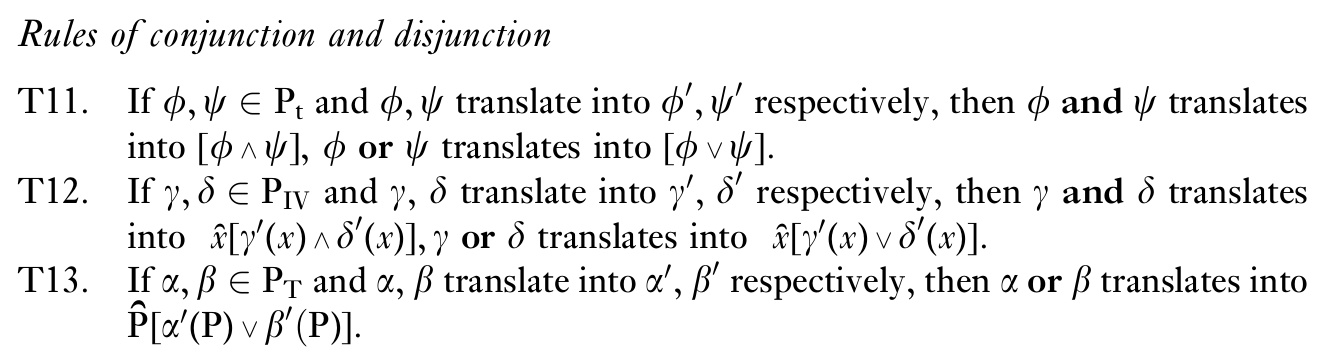
\includegraphics[trim=0 0 0 80,clip,width=0.7\textwidth]{fig/montague-tptoqioe.png}}

        \vspace{1.2em}
        Claim: That doesn't scale well $\leadsto$ \textbf{We need {\color{hlfont}prototyping}!}
    }

    % \newcommand\VP{\text{\upshape\tiny VP}}
    % \hspace{2em}$\llbracket\text{\strplain{$P_{\VP}$ and $Q_{\VP}$}}\rrbracket_{\VP} = \lambda x. \llbracket\text{\strplain{$P_{\VP}$}}\rrbracket(x) \wedge \llbracket\text{\strplain{$Q_{\VP}$}}\rrbracket(x)$
\end{frame}

\begin{frame}
    \frametitle{NLU Prototyping}
    \begin{itemize}
        \item Traditionally done in Prolog/Haskell
        \begin{itemize}
            \item[$\raa$] requires a lot of work
        \end{itemize}
            \item A dedicated framework might be better
        \begin{itemize}
            \item[$\raa$] only partial solutions exist
        \end{itemize}
        \item Can we combine existing partial solutions?\com{Research Question}
        \begin{itemize}
            \item[$\leadsto$] GLIF
        \end{itemize}
    \end{itemize}
\end{frame}

\begin{frame}
    \frametitle{GLIF: Grammatical Logical Inference Framework}
    \centering

%     \parbox[t][1em][t]{\textwidth}{
%         \centering\textit{
%             \only<1-2>{We have a tool for this!}
%             \only<3>{It combines existing tools.}
%         }
%     }

    \vspace{1.5em}
    \only<1-1>{\disablepart{sempragarrow}}
    \only<1-2>{\disablepart{includejupyter}}
    \only<1-2>{\disablepart{gfbox}\disablepart{mmtbox}\disablepart{elpibox}}
    \includestandalone[width=\textwidth]{fig/glif-architecture}

    \vspace{1em}
    \begin{minipage}[t][2cm]{\textwidth}
        \only<1-2>{
            \begin{tikzpicture}
                \node(str) at (-4,0) {\str{Ahmed and Berta paint.}};
                % REQUIRES \usepackage{tikz-qtree}
                \node(ast) at (0,0) {\color{nlfont!50!logicfont}
                    \resizebox{1.5cm}{!}{\tikzset{edge from parent/.append style={very thick}}
                    \Tree [ .\textbf{mkS} [ .\textbf{andNP} [ \textbf{Ahmed} \textbf{Berta} ] ] \textbf{paint} ]
                    }};
                \node(log) at (2.8,0) {\color{logicfont}$p(a) \wedge p(b)$};
                \draw[-{Straight Barb[length=6.3,width=5.0]},gray] (str) -- (ast);
                \draw[-{Straight Barb[length=6.3,width=5.0]},gray] (ast) -- (log);
            \end{tikzpicture}
        }
        \only<3>{
            \setlength{\arrayrulewidth}{1.0pt}
            \begin{tabular}{r@{\hskip3pt} l l}
                \vspace{0.1em} &\textbf{GF}   &{(= \textbf{grammar} framework)}\\
                \vspace{0.1em}+&\textbf{MMT}  &{(= \textbf{logic} framework)}\\
                \vspace{0.1em}+&\textbf{ELPI} &{(= \textbf{inference} framework)}\\
                \hline
                \\[-1em]
                =&\textbf{GLIF} &{(= \textbf{natural language understanding} framework)}\\
                \end{tabular}
        }
    \end{minipage}
\end{frame}
